
\documentclass[twoside,11pt]{homework}
\usepackage{graphicx}
\usepackage{listings}
\usepackage{color}
\definecolor{dkgreen}{rgb}{0,0.6,0}
\definecolor{gray}{rgb}{0.5,0.5,0.5}
\definecolor{mauve}{rgb}{0.58,0,0.82}
\lstset{ %
	language=R,                     % the language of the code
	basicstyle=\footnotesize,       % the size of the fonts that are used for the code
	numbers=left,                   % where to put the line-numbers
	numberstyle=\tiny\color{gray},  % the style that is used for the line-numbers
	stepnumber=1,                   % the step between two line-numbers. If it's 1, each line
	% will be numbered
	numbersep=5pt,                  % how far the line-numbers are from the code
	backgroundcolor=\color{white},  % choose the background color. You must add \usepackage{color}
	showspaces=false,               % show spaces adding particular underscores
	showstringspaces=false,         % underline spaces within strings
	showtabs=false,                 % show tabs within strings adding particular underscores
	frame=single,                   % adds a frame around the code
	rulecolor=\color{black},        % if not set, the frame-color may be changed on line-breaks within not-black text (e.g. commens (green here))
	tabsize=2,                      % sets default tabsize to 2 spaces
	captionpos=b,                   % sets the caption-position to bottom
	breaklines=true,                % sets automatic line breaking
	breakatwhitespace=false,        % sets if automatic breaks should only happen at whitespace
	title=\lstname,                 % show the filename of files included with \lstinputlisting;
	% also try caption instead of title
	keywordstyle=\color{blue},      % keyword style
	commentstyle=\color{dkgreen},   % comment style
	stringstyle=\color{mauve},      % string literal style
	escapeinside={\%*}{*)},         % if you want to add a comment within your code
	morekeywords={*,...},            % if you want to add more keywords to the set
	belowcaptionskip=0em,
	belowskip=0em
} 

\usepackage{etoolbox}
\makeatletter
\patchcmd{\@verbatim}
{\verbatim@font}
{\verbatim@font\footnotesize}
{}{}
\preto{\@verbatim}{\topsep=0pt \partopsep=0pt }
\makeatother

\coursename{COMS 4771 Machine Learning } % DON'T CHANGE THIS

\studname{Jun Hu}    % YOUR NAME GOES HERE
\studmail{jh3846@columbia.edu}% YOUR UNI GOES HERE
\hwNo{1}                   % THE HOMEWORK NUMBER GOES HERE
\collab{}   % THE UNI'S OF STUDENTS YOU DISCUSSED WITH

% Uncomment the next line if you want to use \includegraphics.\textbf{\textbf{\textbf{}}}
%\usepackage{graphicx}

\begin{document}
\maketitle

\section*{Problem 1}

	\begin{enumerate}
		
		\item[\textbf{(a)}] First of all, to numerically summarize, execute:
		
		\begin{lstlisting}
library(ISLR)
summary(Weekly)
		\end{lstlisting}
		
		\begin{verbatim}
		       Year           Lag1               Lag2               Lag3               Lag4         
		  Min.   :1990   Min.   :-18.1950   Min.   :-18.1950   Min.   :-18.1950   Min.   :-18.1950  
		  1st Qu.:1995   1st Qu.: -1.1540   1st Qu.: -1.1540   1st Qu.: -1.1580   1st Qu.: -1.1580  
		  Median :2000   Median :  0.2410   Median :  0.2410   Median :  0.2410   Median :  0.2380  
		  Mean   :2000   Mean   :  0.1506   Mean   :  0.1511   Mean   :  0.1472   Mean   :  0.1458  
		  3rd Qu.:2005   3rd Qu.:  1.4050   3rd Qu.:  1.4090   3rd Qu.:  1.4090   3rd Qu.:  1.4090  
		  Max.   :2010   Max.   : 12.0260   Max.   : 12.0260   Max.   : 12.0260   Max.   : 12.0260  
		       Lag5              Volume            Today          Direction 
		  Min.   :-18.1950   Min.   :0.08747   Min.   :-18.1950   Down:484  
		  1st Qu.: -1.1660   1st Qu.:0.33202   1st Qu.: -1.1540   Up  :605  
		  Median :  0.2340   Median :1.00268   Median :  0.2410             
		  Mean   :  0.1399   Mean   :1.57462   Mean   :  0.1499             
		  3rd Qu.:  1.4050   3rd Qu.:2.05373   3rd Qu.:  1.4050             
		  Max.   : 12.0260   Max.   :9.32821   Max.   : 12.0260 
		
		\end{verbatim}
		
		To graphically summarize, execute:
		
		\begin{lstlisting}
pairs(Weekly)
		\end{lstlisting}
		
		\begin{center}
		  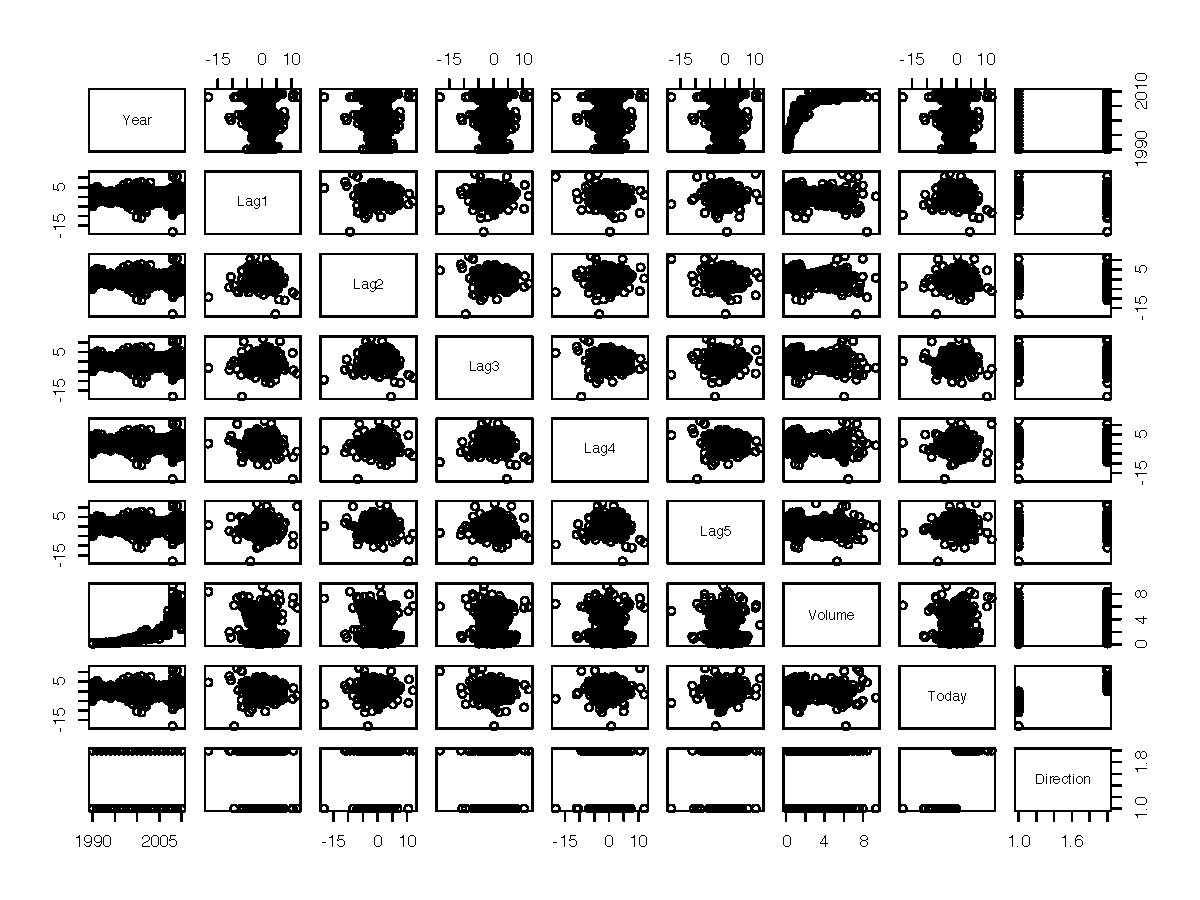
\includegraphics[height=0.5\textheight]{f1.pdf}
		\end{center}
		
		To observe all pairwise correlations, execute:
		
		\begin{lstlisting}
cor(Weekly[, -9])
		\end{lstlisting}
		
		\begin{verbatim}
		               Year         Lag1        Lag2        Lag3         Lag4         Lag5      Volume
		 Year    1.00000000 -0.032289274 -0.03339001 -0.03000649 -0.031127923 -0.030519101  0.84194162
		 Lag1   -0.03228927  1.000000000 -0.07485305  0.05863568 -0.071273876 -0.008183096 -0.06495131
		 Lag2   -0.03339001 -0.074853051  1.00000000 -0.07572091  0.058381535 -0.072499482 -0.08551314
		 Lag3   -0.03000649  0.058635682 -0.07572091  1.00000000 -0.075395865  0.060657175 -0.06928771
		 Lag4   -0.03112792 -0.071273876  0.05838153 -0.07539587  1.000000000 -0.075675027 -0.06107462
		 Lag5   -0.03051910 -0.008183096 -0.07249948  0.06065717 -0.075675027  1.000000000 -0.05851741
		 Volume  0.84194162 -0.064951313 -0.08551314 -0.06928771 -0.061074617 -0.058517414  1.00000000
		 Today  -0.03245989 -0.075031842  0.05916672 -0.07124364 -0.007825873  0.011012698 -0.03307778
		               Today
		 Year   -0.032459894
		 Lag1   -0.075031842
		 Lag2    0.059166717
		 Lag3   -0.071243639
		 Lag4   -0.007825873
		 Lag5    0.011012698
		 Volume -0.033077783
		 Today   1.000000000
		
		\end{verbatim}
		
		We found that there exists a higher correlation of 0.84 between Year and Volume, while others are pretty low. Also from the plot we can recognize there is an increasingly correlated pattern between Year and Volume.
		
		
		\item[\textbf{(b)}] Execute:
		
		\begin{lstlisting}
glm.fit = glm(Direction~., data=Weekly[, c(2:7, 9)], family=binomial)
summary(glm.fit)
		\end{lstlisting}
		
		\begin{verbatim}
		Call:
		glm(formula = Direction ~ ., family = binomial, data = Weekly[, 
		    c(2:7, 9)])
		
		Deviance Residuals: 
		    Min       1Q   Median       3Q      Max  
		-1.6949  -1.2565   0.9913   1.0849   1.4579  
		
		Coefficients:
		            Estimate Std. Error z value Pr(>|z|)   
		(Intercept)  0.26686    0.08593   3.106   0.0019 **
		Lag1        -0.04127    0.02641  -1.563   0.1181   
		Lag2         0.05844    0.02686   2.175   0.0296 * 
		Lag3        -0.01606    0.02666  -0.602   0.5469   
		Lag4        -0.02779    0.02646  -1.050   0.2937   
		Lag5        -0.01447    0.02638  -0.549   0.5833   
		Volume      -0.02274    0.03690  -0.616   0.5377   
		---
		Signif. codes:  0 ‘***’ 0.001 ‘**’ 0.01 ‘*’ 0.05 ‘.’ 0.1 ‘ ’ 1
		
		(Dispersion parameter for binomial family taken to be 1)
		
		    Null deviance: 1496.2  on 1088  degrees of freedom
		Residual deviance: 1486.4  on 1082  degrees of freedom
		AIC: 1500.4
		
		Number of Fisher Scoring iterations: 4
		
		\end{verbatim}
		
		From the summary, it seems Lag2 has statistical significance.
		
		\item[\textbf{(c)}] Execute:
		
		\begin{lstlisting}
glm.probs = predict(glm.fit, type = "response")
glm.pred = ifelse(glm.probs>0.5, "Up", "Down")
table(glm.pred, Weekly$Direction)
		\end{lstlisting}
		
		\begin{verbatim}
		glm.pred Down  Up
		    Down   54  48
		    Up    430 557
		    
		\end{verbatim}
		
		The correct prediction is: accuracy $=\frac{54+557}{54+430+48+557} = 56.11\%$\\
		So the incorrect prediction is: error rate $=1-56.11\%=43.89\%$\\
		These numbers tell us the overall accuracy and error of predictions.\\
		
		The correct market "Down" rate: is: recall $=\frac{54}{54+430}=11.16\%$\\
		So the incorrect market "Down" rate is: miss $=1-11.16\%=88.84\%$\\
		The correct market "Up" rate is: specificity $=\frac{557}{48+557}=92.07\%$\\
		So the incorrect market "Up" rate is: miss $=1-92.07\%=7.93\%$\\
		These numbers tell us when the market goes up, the model can predict correctly in a very high rate, but  quite the contrary when the market goes down.
		
		\item[\textbf{(d)}] Execute:
		
		\begin{lstlisting}
attach(Weekly)
train = (Year<2009)
Weekly.test = Weekly[!train,]
glm.fit = glm(Direction~Lag2, data=Weekly, family=binomial, subset=train)
glm.probs = predict(glm.fit, Weekly.test, type="response")
glm.pred = ifelse(glm.probs>0.5, "Up", "Down")
Direction.test = Direction[!train]
table(glm.pred, Direction.test)
		\end{lstlisting}
		
		\begin{verbatim}
		        Direction.test
		glm.pred Down Up
		    Down    9  5
		    Up     34 56
		    
		\end{verbatim}
		
		The overall correct prediction can be simply calculated by executing:
		
		\begin{lstlisting}
mean(glm.pred==Direction.test)
		\end{lstlisting}
		
		\begin{verbatim}
		[1] 0.625
		
		\end{verbatim}
		
		So the overall accuracy $=62.5\%$.
		
		\item[\textbf{(e)}] Execute:
		
		\begin{lstlisting}
library(MASS)
lda.fit = lda(Direction~Lag2, data=Weekly, subset=train)
lda.pred = predict(lda.fit, Weekly.test)
table(lda.pred$class, Direction.test)
		\end{lstlisting}
		
		\begin{verbatim}
		      Direction.test
		       Down Up
		  Down    9  5
		  Up     34 56
		  
		\end{verbatim}
		
		To get overall correct prediction, execute:
		
		\begin{lstlisting}
mean(lda.pred$class==Direction.test)
		\end{lstlisting}
		
		\begin{verbatim}
		[1] 0.625
		
		\end{verbatim}
		
		The accuracy $=62.5\%$
		
		\item[\textbf{(f)}] Execute(fix result using 'set.seed(23)'):
		
		\begin{lstlisting}
library(class)
train.X = as.matrix(Lag2[train])
test.X = as.matrix(Lag2[!train])
Direction.train = Direction[train]
set.seed(23)
knn.pred = knn(train.X, test.X, Direction.train, k=1)
table(knn.pred, Direction.test)
		\end{lstlisting}
		
		\begin{verbatim}
		         Direction.test
		 knn.pred Down Up
		     Down   21 29
		     Up     22 32
		    
		\end{verbatim}
		
		To get overall correct prediction, execute:
		
		\begin{lstlisting}
mean(knn.pred==Direction.test)
		\end{lstlisting}
		
		\begin{verbatim}
		[1] 0.5096154
		
		\end{verbatim}
		
		The accuracy $=50.96\%$
		
		\item[\textbf{(g)}] The logistic regression model and linear discriminant analysis model appear to provide the best results of the data.
		
		\item[\textbf{(h)}] By using the same train and test sets as above, we can change the predictors and $k$ values to optimize the correct predictions as below:
		
		\textbf{1. logistic regression}\\
		Change predictors to $Lag2+(Lag1)^2$  -- execute the code:\\
		
		\begin{lstlisting}
glm.fit = glm(Direction~Lag2+I(Lag1^2), data=Weekly, family=binomial, subset=train)
glm.probs = predict(glm.fit, Weekly.test, type="response")
glm.pred = ifelse(glm.probs>0.5, "Up", "Down")
table(glm.pred, Direction.test)
		\end{lstlisting}
		
		\begin{verbatim}
       Direction.test
		glm.pred Down Up
   Down    8  2
   Up     35 59
   
		\end{verbatim}
		
		To calculate the current correct prediction:
		
		\begin{lstlisting}
mean(glm.pred==Direction.test)
		\end{lstlisting}
		
		\begin{verbatim}
		[1] 0.6442308
		
		\end{verbatim}
		
		Accuracy $=64.42\%$

		\textbf{2. linear discriminant analysis}\\
		Change predictors to $Lag2+(Lag1)^2$  -- execute the code:\\
		
		\begin{lstlisting}
lda.fit = lda(Direction~Lag2+I(Lag1^2), data=Weekly, subset=train)
lda.pred = predict(lda.fit, Weekly.test)
table(lda.pred$class, Direction.test)
		\end{lstlisting}
		
		\begin{verbatim}
      Direction.test
       Down Up
  Down    8  2
  Up     35 59
   
		\end{verbatim}
		
		To calculate the current correct prediction:
		
		\begin{lstlisting}
mean(lda.pred$class==Direction.test)
		\end{lstlisting}
		
		\begin{verbatim}
		[1] 0.6442308
		
		\end{verbatim}
		
		Accuracy $=64.42\%$
		
		\textbf{3. KNN}\\
		Test k from $1$ to $300$ (fix results by using 'set.seed(23)'):\\
		
		\begin{lstlisting}
k_increasement = data.frame(k=1:300, accuracy=NA)
for (i in 1:300){
  set.seed(23)
  knn.pred = knn(train.X, test.X, Direction.train, k=i)
  table(knn.pred, Direction.test)
  k_increasement$accuracy[i] = mean(knn.pred==Direction.test)
}
		\end{lstlisting}
		
		To calculate the current correct prediction and display as a plot, finally identify the value of $k$ that obtain the best accuracy:
		
		\begin{lstlisting}
plot(x=k_increasement$k, y=k_increasement$accuracy, type='l', xlab="k", ylab="accuracy", ylim=c(0.45, 0.7), lwd=3, col='red')
identify(x=k_increasement$k, y=k_increasement$accuracy, plot=T)
		\end{lstlisting}
		
		\begin{center}
		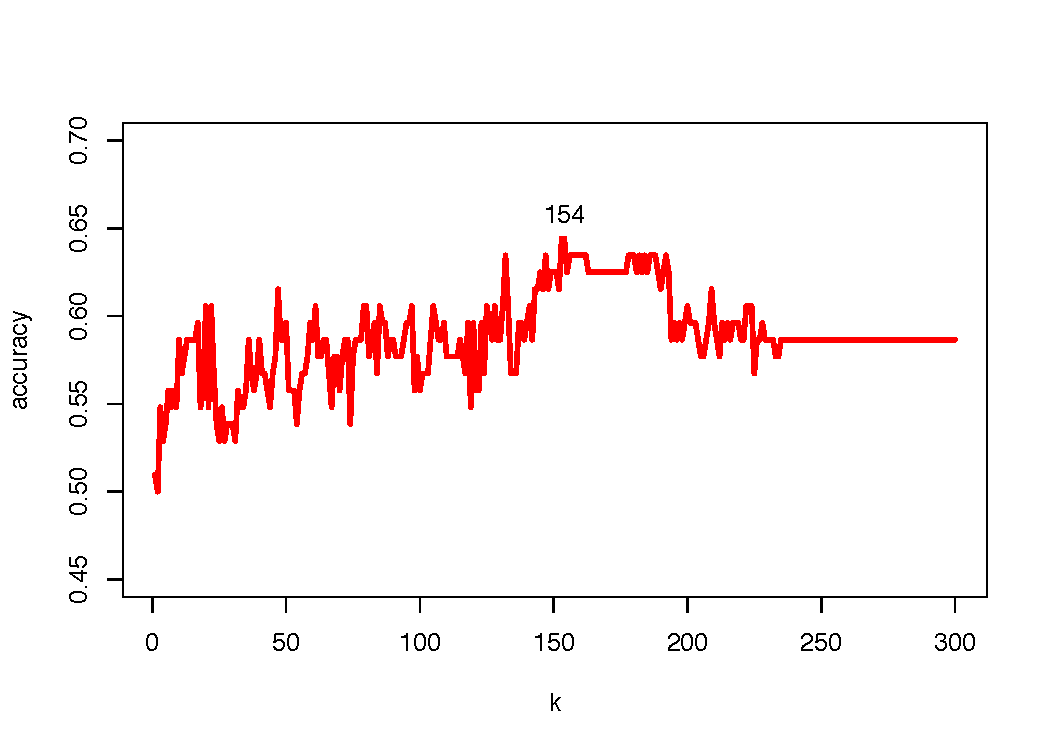
\includegraphics[height=0.5\textheight]{f2.pdf}
		\end{center}
		
		The best correct prediction is at $k=154$, and the this correct prediction can be retrieved as:
		
		\begin{lstlisting}
k_increasement[154,]
		\end{lstlisting}
		
		\begin{verbatim}
		       k  accuracy
		 154 154 0.6442308
		
		\end{verbatim}
		
		Accuracy $=64.42\%$
		
	\end{enumerate}


\section*{Problem 2}

	\begin{align*}
	\mathbb{E}[X] &= \int x p(x) \mathrm{d}x\\
	&= \iint x p(x,y) \mathrm{d}x \mathrm{d}y\\
	&= \iint x  \left( p(x \mid y) p(y) \right) \mathrm{d}x \mathrm{d}y\\
	&= \int \left( \int x  [ p(x \mid y) \mathrm{d}x \right) p(y) \mathrm{d}y\\
	&= \int \left( \mathbb{E}_x[x \mid y] \right) p(y) \mathrm{d}y\\
	&= \mathbb{E}_y[ \mathbb{E}_x[x \mid y] ]\\
	\\
	\mathrm{var} &= \mathbb{E}[x^2] - \mathbb{E}[x]^2\\
	&= \mathbb{E}_y[ \mathbb{E}_x[x^2 \mid y] ]	- ( \mathbb{E}_y[ \mathbb{E}_x[x \mid y] ] )^2\\
	&= \mathbb{E}_y[ \mathbb{E}_x[x^2 \mid y] - \mathbb{E}_x[x \mid y]^2] + \mathbb{E}_y[\mathbb{E}_x[x \mid y]^2]	- ( \mathbb{E}_y[ \mathbb{E}_x[x \mid y] ] )^2\\
	&= \mathbb{E}_y [\mathrm{var}[x \mid y]] + \mathrm{var}_y[\mathbb{E}_x[x \mid y]]
	\end{align*}
	
	
\section*{Problem 3}

Because $y=x+z$, and $x$ and $y$ having Gaussian distributions, which means we have the distributions as below:

	\begin{align}
	p(x) &= \mathcal{N} (x \mid \mu_x, \Sigma_x)\\
	p(y \mid x) &= \mathcal{N} (y \mid \mu_z+x, \Sigma_z)
	\end{align}
	
Compare (1) and (2) to (2.99) and (2.100), we can have:
	\begin{align}
\mu=\nu_x, \Lambda^{-1}=\Sigma_x, A=1, b=\mu_z, L^{-1}=\Sigma_z
	\end{align}
	
Because of (2.109) and (2.110), we can have:
	\begin{align}
		p(y \mid x) &= \mathcal{N} (\mathbb{E}[y], \mathrm{cov}[y])\\
		&= \mathcal{N} (A\mu+b, L^{-1}+A\Lambda^{-1}A^T)
	\end{align}

Use (3) in (5), we can find the marginal distribution $p(y)$:
$$p(y)= \mathcal{N} (y \mid \mu_x+\mu_z, \Sigma_x+\Sigma_z)$$

\section*{Problem 4}

The data are linearly separable and the decision boundary is 0, which means separate these two classes by the hyperplane with corresponding $\sigma = 0.5$, that is $w^T\phi=0$, which implies $w$ goes to infinite. And logistic sigmoid becomes infinite steep. Or we see any other logistic function which decreases less sharply would give a lower maximum likelihood. However, whenever a posterior probability reaches $1$, any function which passes through the data points would give the same likelihood. As there is no closed-form for the maximum likelihood,  when we trying to estimate the optimal $w$, there will be infinite magnitude.

\section*{Problem 5}

Since this is a binary classification problem, generally for data point $\{x_i, t_i\}$, if $t_i=1$ for $p$, then $t_i=0$ for $1-p$, then we can have the likelihood (6) and its "$\log$" form (7):
	\begin{align}
	&\prod_{i=1}^N p(x_i)^{t_i}(1-p(x_i)^{1-t_i} \\
	&\sum_{i=1}^{N} t_i \log p(x_i) + (1-t_i) \log (1-p(x_i))
	\end{align}
	
In this specified problem, having instead a value $\pi_n$ representing the probability that $t_n=1$, which means $t_i$ is substituted by $\pi_i$. Moreover, given the probability model $p(1 \mid \phi)$, we can have that $p(x_i)$ is given by $p(t_i =1 \mid \phi(x_i))$. That is:

	\begin{align}
	t_i  &\longrightarrow \pi_i\\
	p(x_i) &\longrightarrow p(t_i =1 \mid \phi(x_i))
	\end{align}

Use (8) and (9) in (7), we can have the $\log$ likelihood for this specified data:

$$
\sum_{i=1}^{N} \pi_i\log p(t_i =1 \mid \phi(x_i)) + (1-\pi_i) \log (1-p(t_i =1 \mid \phi(x_i)))
$$


\end{document} 
